\section{Hardware}

\subsection{Arten von VR Headsets}\label{sec:vr-headset-types}

\subsubsection{Tethered VR Headsets}

\subsubsection{Standalone VR Headsets}

\subsubsection{Smartphone VR and handheld VR viewers}

\subsection{VR Headset}\label{sec:vr-headset}

VR Headsets gibt es auf dem Markt schon viele.
Nach einer Statistik in 2017 sind die beliebtesten VR Headset Hersteller Sony, Oculus und HTC (Siehe Abbildung~\ref{fig:vr_headset_manufacturer_marketshare}).

\begin{figure}
    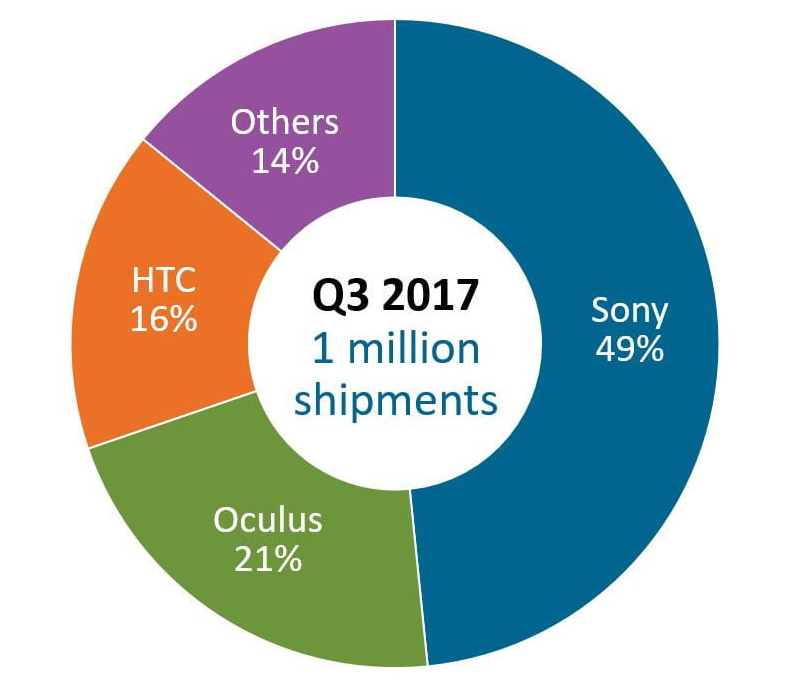
\includegraphics[scale=0.5]{pics/vr_headset_manufacturer_marketshare}
    \caption{Market-share VR Headset Hersteller~\cite{MARTINDALE_2017}}
    \label{fig:vr_headset_manufacturer_marketshare}
\end{figure}

\subsubsection{HTC Vive Pro}

Wie bereits in Abschnitt~\ref{sec:vr-headset-types} beschrieben, gibt es von diesen Headsets verschiedene Arten.
Die HTC Vive Pro ist vom Typ ein tethered Headset mit dem Zusatz, dass auch sogenannte Light Houses gebraucht werden (Siehe Abschnitt~\ref{sec:lighthouse}).
Andere Produkte, wie die im nächsten Abschnitt beschriebene Oculus Quest benötigen diese nicht.

\paragraph{Vorteile}

\begin{itemize}
    \item {\bf Einfache Verwaltung} Die HTC kann mit SteamVR verwalted werden, womit der manuelle Download von externer Software vermieden wird.
    \item genaueres Tracking mit externen Sensoren~\ref{sec:lighthouse}
    \item leichtes einbinden von SteamVR kompatiblen Trackern
\end{itemize}

\paragraph{Nachteile}

\begin{itemize}
    \item langer Aufbau
    \begin{itemize}
        \item anstecken des VR Headsets
        \item aufbauen der sensoren~\ref{sec:lighthouse}
        \item Synchronisierung der Sensoren
        \item mögliches aufsetzen von zusätzlichen Trackern
    \end{itemize}
\end{itemize}


\subsubsection{Oculus Quest 2}\label{sec:oculus-quest-2}

\subsection{VR Controller}\label{sec:vr-controller}

\subsection{Tracker}\label{sec:tracker}

\subsubsection{Vive Tracker}\label{sec:vive-tracker}

\subsection{Lichtboxen}\label{sec:lighthouse}

\subsection{Wireless Adapter }

\section{Software}

\subsection{Game Engine}

Es gibt mehrere Games Engines mit welchen eine VR Applikation entwickelt werden kann.
In Abbildung~\ref{fig:game_engine_marketshare} kann man den Marktanteil verschiedener Engines sehen.
Diese Daten sind aber mit Vorsicht zu genießen, da das Skript welche diese Daten geliefert hat nach einigen Kriterien handelt, siehe~\cite{REDDIT_2018}.
Auf Basis dieser Statistik werden die drei Engines mit dem höchsten Marktanteil vorgestellt.
id Tech, welche auf Basis der reinen Zahlen die drittgrößte Engine wäre, wurde hier ausgenommen.

\begin{figure}
    \centering
    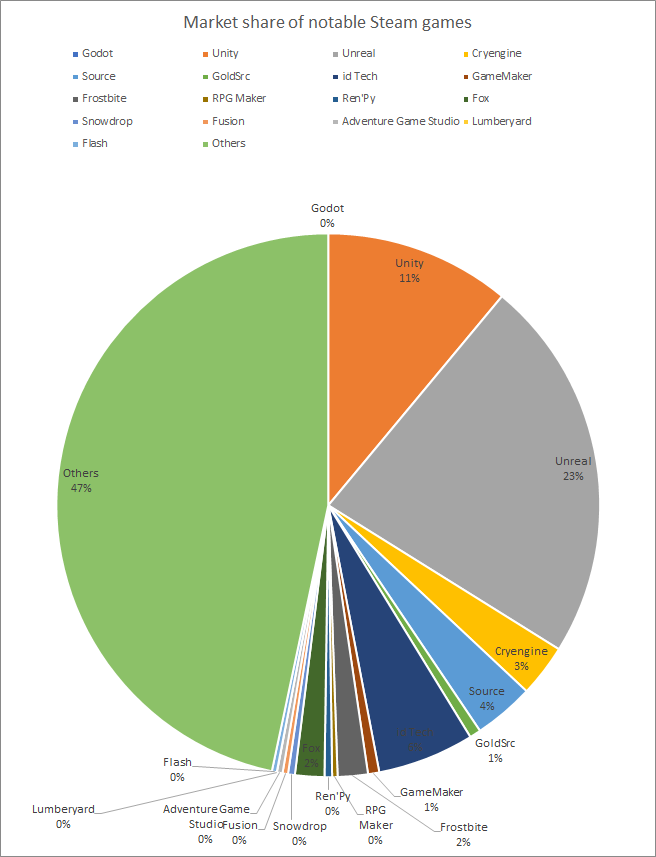
\includegraphics[scale=0.4]{pics/game_engine_marketshare}
    \caption{Game Engine Market-share~\cite{REDDIT_2018}}
    \label{fig:game_engine_marketshare}
\end{figure}

\begin{figure}
    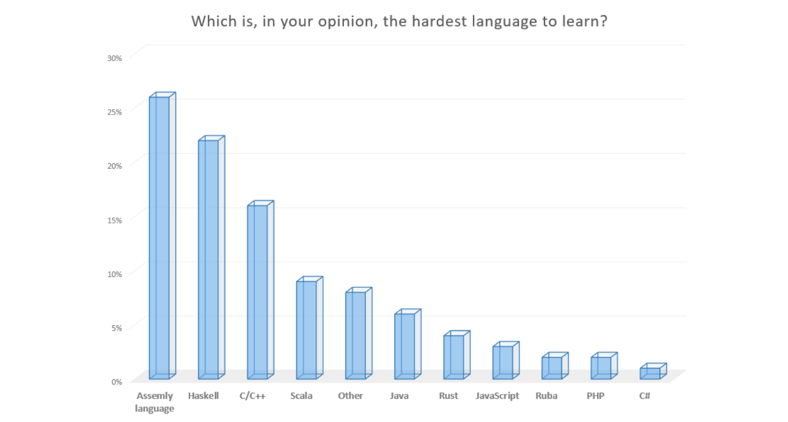
\includegraphics[scale=0.4]{pics/programming_languages_hardest}
    \caption{Schwerste Programmiersprachen~\cite{JAXCENTER_2018}}
    \label{fig:hardest_programming_languages}
\end{figure}

\subsubsection{Unity}

Unity ist eine Game Engine, welche von Unity Technologies initial exklusiv für Apple Mac OS X entwickelt wurde.
Die Engine wurde portiert und kann heute auch auf Windows und auf der Linux Plattform benützt werden.
Die Engine ist für Einsteiger gratis.
Auch wenn sie eine Einsteiger Engine genannt wird, wird sie trotzdem im professionellen Bereich genutzt und viele bekannte Spiele wurden mit Unity entwickelt.
Spiele wie Pokemon GO, Among us und Hearthstone wurden in der Unity Engine entwickelt~\cite{Haas2014AHO,UNITY_DOWNLOAD,UNITY_PRICING,WIKIPEDIA_UNITY_GAME_LIST_2014}.

\paragraph{Vorteile}

\begin{itemize}
    \item Gratis Lizenz für persönlichen Nutzen und für Unternehmen mit unter 100.000 \$ Einkommen~\cite{UNITY_PRICING}
    \item Programmierbar in C\#~\ref{fig:hardest_programming_languages}
    \item Es kann für alle möglichen Plattformen ein Programm geschrieben werden~\cite{UNITY_PLATTFORMS}
    \begin{itemize}
        \item IOS
        \item Android
        \item Windows
        \item Linux
        \item WebGL
        \item usw.
    \end{itemize}
\end{itemize}

\paragraph{Nachteile}

\begin{itemize}
    \item weniger Market-share~\ref{fig:game_engine_marketshare}
    \item geschlossener Source Code
    \item schnellerer Kostenanfall wie z.B.\ bei~\ref{sec:unreal_engine}
\end{itemize}

\subsubsection{Unreal Engine}
\label{sec:unreal_engine}

Unreal Engine ist von Epic Games entwickelt~\cite{UNEAL_ENGINE_OWNER_2022}.
Diese Engine ist eine weit verwendete Game Engine.
Dies kann man auch in Abbildung~\ref{fig:game_engine_marketshare} herausnehmen.
Viele Spiele wie Fortnite, Ark Survival Evolved, Borderlands 3 und Jedi Fallen Order sind mit dieser Engine entwickelt worden~\cite{WIKIPEDIA_UNREAL_GAME_LIST}.

\begin{figure}
    \centering
    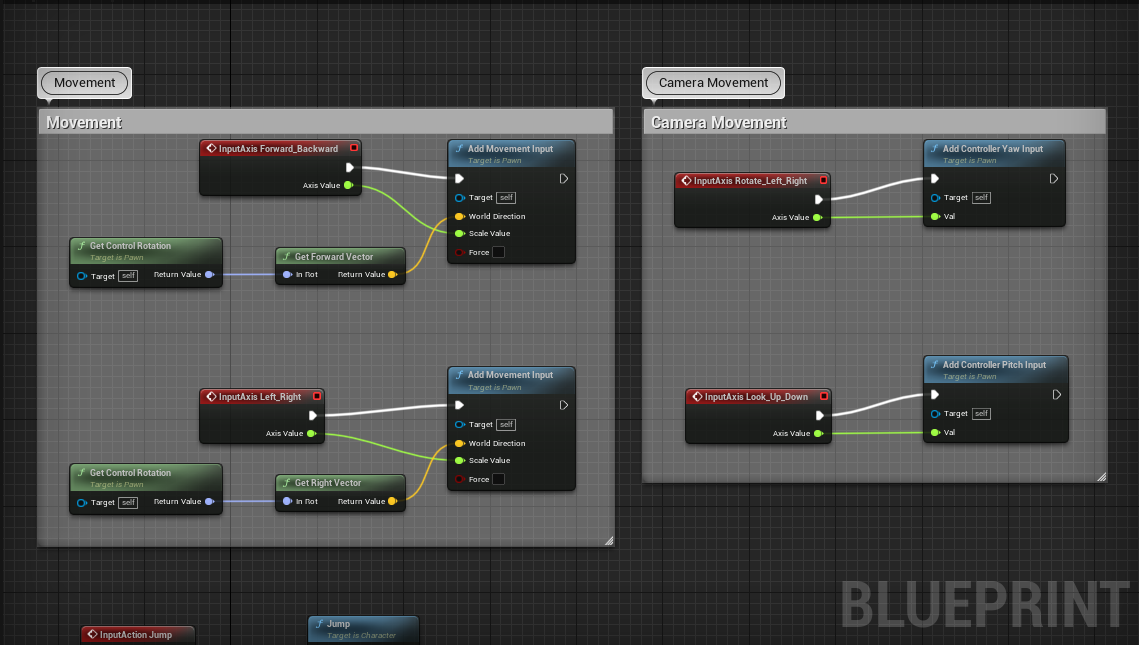
\includegraphics[scale=0.3]{pics/visual_scripting_unreal_engine}
    \caption{Visual Scripting in Unreal Engine 5}
    \label{fig:visual_scripting_unreal_engine}
\end{figure}

\paragraph{Vorteile}

\begin{itemize}
    \item großer Market-share~\ref{fig:game_engine_marketshare}
    \item 'easy to learn' visual scripting~\ref{fig:visual_scripting_unreal_engine}
    \item Nutzungshonorar von 5\% tritt erst bei einem Einkommen von einem Produkt von 1.000.000\$~\cite{UNREAL_ENGINE_PRICING_2022}
\end{itemize}

\paragraph{Nachteile}

\begin{itemize}
    \item 5\% Nutzungshonorar, wenn das Einkommen eines Produktes über 1000000\$ ist~\cite{UNREAL_ENGINE_PRICING_2022}
    \item für erweiterte funktionalität wird c++ welches nach Umfrage in der Abbildung~\ref{fig:hardest_programming_languages} die dritt schwierigste Sprache ist
\end{itemize}

\subsubsection{Source Engine und Source 2 Engine}

Es gibt mittlerweile 2 Iterationen dieser Engine.
Zum einen die originale Source Engine und die Source Engine 2.
Die Markteinführung von der originalen Source Engine war im Juni 2004~\cite{Bryan_Wirtz_SOURCE_ENGINE_2022}.
Daraufhin ist die Source 2 Engine im August 2014 herausgekommen~\cite{VALVE_DEVELOPER_COMMUNITY_SOURCE2}.
Beider dieser Engines sind von Valve entwickelt worden~\cite{VALVE_DEVELOPER_COMMUNITY_SOURCE, VALVE_DEVELOPER_COMMUNITY_SOURCE2}.
Verantwortlich ist die Source 2 Engine für Spiele wie Dota 2 und Half Life Alyx~\cite{WIKIPEDIA_SOURCE2_ENGINE_GAME_LIST}.
Andere Spiele wie Half Life 2, Counterstrike Source, Portal, Portal 2 und Counterstrike Global Offensive sind mit der originalen Source Engine entwickelt worden~\cite{WIKIPEDIA_SOURCE_ENGINE_GAME_LIST}.
Auch als VR Entwicklungsumgebung eignet es sich, da sie für Half Life: Alyx eines der erfolgreichsten VR Spiele benutzt worden ist~\cite{WIKIPEDIA_SOURCE2_ENGINE_GAME_LIST, Aden_Carter_2020}.
Die kommenden Vorteile und Nachteile handeln sich um die Source 2 Engine.

\paragraph{Vorteile}

\begin{itemize}
    \item Source Engine ist gratis zu nutzen und zu publizieren *~\ref{pgr:cons}
\end{itemize}


\paragraph{Nachteile}\label{pgr:cons}

\begin{itemize}
    \item kein hoher Market-share (siehe Abbildung~\ref{fig:game_engine_marketshare})
    \item Spiele müssen auf Steam publiziert werden~\cite{Brenna_Hillier_2015}
\end{itemize}



\subsection{VR Plugin}

\subsection{Steam}

\subsection{Vive Wireless}

\subsection{Final IK Plugin}

\subsection{IDE}

\subsection{Modellierung}
